\chapter{Wellen in einem Kanal\label{chapter:wellen}}
\lhead{Wellen in einem Kanal}
\begin{refsection}
\chapterauthor{Daniela Meier und Hansruedi Patzen}
\clearpage

Das Kapitel \ref{chapter:wellen} Wellen besch"aftigt sich mit Ausbreitung von 
Wellen in einem 
parabolischen Kanal. Die Ausbreitung wird mittels Analyse der Wellengleichung 
n"aher betrachtet. In einem ersten Schritt wird erkl"art, wie die 
Gleichung\ref{wellen:grundgleichung} aus der Aufgabenstellung zustandegekommen 
ist.

\begin{equation}
	y'' + (ax^2+bx+c)y
	=
	0
	\label{wellen:grundgleichung}
\end{equation}

Die allgemeine Differentialgleichung der Welle lautet (gem"ass 
\cite{wellen:smirnow2}):

\begin{equation}
	\frac{\partial^2 u}{\partial t^2}
	=
	c^2
	\left(
		\frac{\partial^2 u}{\partial x^2} 
		+ \frac{\partial^2 u}{\partial y^2} 
		+ \frac{\partial^2 u}{\partial z^2}
	\right)
	\label{wellen:allgemeineDGL}
\end{equation}

Da in der ausgew"ahlten Problemstellung nur eine zweidimensionale Welle 
betrachtet wird, fallen die y- und die z-Koordinate weg. Die Gleichung 
vereinfacht sich dadurch zu:

\begin{equation}
	\frac{\partial^2 u}{\partial t^2}
	=
	c^2
	\left(
		\frac{\partial^2 u}{\partial x^2} 
	\right)
	\label{wellen:allgemeineDGLvereinfacht}
\end{equation}

Somit ist die Funktion u noch abh"angig von der Zeit $t$ und der Ortskoordinate 
$x$.

\begin{equation}
	u = f(x,t)
\end{equation}

Zur L"osung der vereinfachten Wellengleichung 
\ref{wellen:allgemeineDGLvereinfacht} wird die Theorie des Separationsansatzes 
verwendet. Gem"ass dem Ansatz kann die Funktion $u$ in ein Produkt zweier 
Funktionen $X(x)$ und $T(t)$ umgewandelt werden.

\begin{equation}
	u (x,t) = X(x) T(t)
	\label{wellen:separierteFunktion}
\end{equation}

Ausgehend von der Grundgleichung der Welle 
\ref{wellen:allgemeineDGLvereinfacht} wird die Funktion 
\ref{wellen:separierteFunktion} auf der linken Seite zweimal partiell nach t 
und auf der rechten Seite zweimal partiell nach x abgeleitet. Daraus resultiert:

\begin{equation}
	T''(t) X(x) = c^2 X''(x)T(t)
\end{equation}

Diese Differentialgleichung wird nun durch $T(x)X(x)$ dividiert und somit 
werden die Variablen separiert und ein Term entsteht, welcher nur funktioniert, 
wenn beide Seiten der Gleichung konstant sind. 

\begin{equation}
	\frac{T''(t)}{T(t)}
	=
	c^2 \frac{X''(x)}{X(x)} = konstant = \lambda
\end{equation}

Aus dieser Gleichung entstehen nun zwei l"osbare Differentialgleichungen 
zweiter Ordnung.

\begin{equation}
	T''= \lambda T(t)
\end{equation}

\begin{equation}
	X''=\frac{\lambda}{c^2}X(x)
	\label{wellen:DGLzweiterOrdnung}
\end{equation}

Bei der Problemstellung, die betrachtet wird, wird davon ausgegangen, dass die 
Zeit konstant ist. Aus diesem Grund wird ab hier nur weiter auf die Gleichung 
der Funktion X(x) eingegangen. Wird die Gleichung 
\ref{wellen:DGLzweiterOrdnung} zu Null gesetzt ergibt sich:

\begin{equation}
	X''(x) -
	\frac{\lambda}{c^2} X(x)
	=0
\end{equation}

Diese Gleichung widerspiegelt die Wellengleichung, die in der Fortsetzung 
betrachtet wird. 

Mit dem Faktor $-\frac{\lambda}{c^2}$ k"onnen verschiedene 
Geschwindigkeitsprofile betrachtet werden. Hier wird zuerst auf den speziellen 
Fall eines parabolischen Profils eingegangen. Die zu untersuchende 
Differentialgleichung ergibt sich hiermit zu der am Anfang definierten 
Gleichung \ref{wellen:grundgleichung}, mit den frei w"ahlbaren Variablen 
${a,b,c} \in \mathbb{R}$, sowie $y(x) = a_0$ und $y'(x) = a_1$.

\section{Potenzreihenl"osung}
Als L"osungsansatz wird der im Kapitel \ref{chapter:potenzreihen} 
kennengelernte Potenzreihenansatz (\ref{potenzreihen:ansatz}) verwendet.

Zuerst werden die Potenzreihen f"ur $y$ und $y''$ aufgestellt.

\begin{equation}
	y(x)
	=
	\sum_{k = 0}^{\infty} a_{k}x^k
	=
	a_0 + a_1x + a_2x^2 + a_3x^3 + a_4x^4 + a_5x^5 + a_6x^6 + \dotsb
	\label{wellen:ersteableitung}
\end{equation}

\begin{equation}
	y''(x)
	=
	\sum_{k = 0}^{\infty} a_{k+2}(k+1)(k+2)x^k
	=
	2a_2 + 3 \mathbin{\cdot} 2a_3x + 4 \mathbin{\cdot} 3a_4x^2 + 5 
	\mathbin{\cdot} 4a_5x^3 + 6 \mathbin{\cdot} 5a_6x^4 + \dotsb
	\label{wellen:zweiteableitung}
\end{equation}

Aus den beiden Gleichungen \ref{wellen:ersteableitung} und 
\ref{wellen:zweiteableitung} kann nun der Koeffizientenvergleich 
\ref{wellen:koeffizietenvergleich} erstellt werden.

\begin{equation}
	\begin{split}
		y''
		&=
		-(ax^2+bx+c)y \\
		2a_2 + 3 \mathbin{\cdot} 2a_3x + 4 \mathbin{\cdot} 3a_4x^2 + \dotsb
		&=
		-(ax^2+bx+c)(a_0 + a_1x + a_2x^2 + a_3x^3 + a_4x^4 + \dotsb) \\
		2a_2 + 3 \mathbin{\cdot} 2a_3x + 4 \mathbin{\cdot} 3a_4x^2 + \dotsb
		&=
		-aa_0x^2-aa_1x^3-aa_2x^4-\dotsb \\
		&\hspace{10pt}
		-ba_0x-ba_1x^2-ba_2^3-ba_3x^4-\dotsb \\
		&\hspace{10pt}
		-ca_0-ca_1x-ca_2x^2-ca_3x^3-ca_4x^4 - \dotsb
	\end{split}
	\label{wellen:koeffizietenvergleich}
\end{equation}

Daraus resultieren nun die Resultate f"ur die verschiedenen $a_k$.

\begin{equation}
	\begin{split}
		a_2
		&=
		-\frac{1}{2}ca_0 \\
		a_3
		&=
		-\frac{1}{3 \cdot 2} (ba_0 + ca_1) \\
		a_4
		&=
		-\frac{1}{4 \cdot 3} (aa_0 + ba_1 + ca_2) \\
		&=
		-\frac{1}{4 \cdot 3} (aa_0 + ba_1 -\frac{1}{2}c^2a_0) \\
		a_5
		&=
		-\frac{1}{5 \cdot 4} (aa_1 + ba_2 + ca_3) \\
		&=
		-\frac{1}{5 \cdot 4} (aa_1 -\frac{1}{2}bca_0 -\frac{1}{3 \cdot 2} 
		c(ba_0 + ca_1)) \\
		&\hspace{5pt}\vdots
	\end{split}
	\label{wellen:aks}
\end{equation}

Hieraus l"asst sich nun eine allgemeine Rekursionsformel 
\ref{wellen:koeffizientengleichung} f"ur die verschiedenen $a_k$ herauslesen. 
Es gilt: $k \in \mathbb{N}_0$ und	$a_{k < 0} = 0$

\begin{equation}
	a_{k+2} = -\frac{1}{(k+2)(k+1)} (aa_{k-2}+ba_{k-1}+ca_k)
	\label{wellen:koeffizientengleichung}
\end{equation}

Nun kann man die L"osungsgleichung \ref{wellen:ygleichung} f"ur $y(x)$ 
herstellen.

\begin{equation}
	y(x) = a_0 + a_1x 
	-\sum_{k=0}^{\infty}\frac{1}{(k+2)(k+1)}(aa_{k-2}+ba_{k-1}+ca_k)x^{k+2}
	\label{wellen:ygleichung}
\end{equation}

Um das Programmieren dieser Formel zu vereinfachen, formt man sie am besten von 
$a_{k+2}$ nach $a_k$ um. Damit erh"alt man die Gleichung 
\ref{wellen:koeffizientengleichungak}.
Bei der neuen $y(x)$-Gleichung \ref{wellen:ygleichungak} muss nun aber $k \in 
\mathbb{N} \backslash \{0, 1\}$ gelten.

\begin{equation}
	a_{k} = -\frac{1}{k(k-1)} (aa_{k-4}+ba_{k-3}+ca_{k-2})
	\label{wellen:koeffizientengleichungak}
\end{equation}

\begin{equation}
	y(x) = a_0 + a_1x 
	-\sum_{k=2}^{\infty}\frac{1}{k(k-1)}(aa_{k-4}+ba_{k-3}+ca_{k-2})x^k
	\label{wellen:ygleichungak}
\end{equation}

\section{Graphische L"osung}
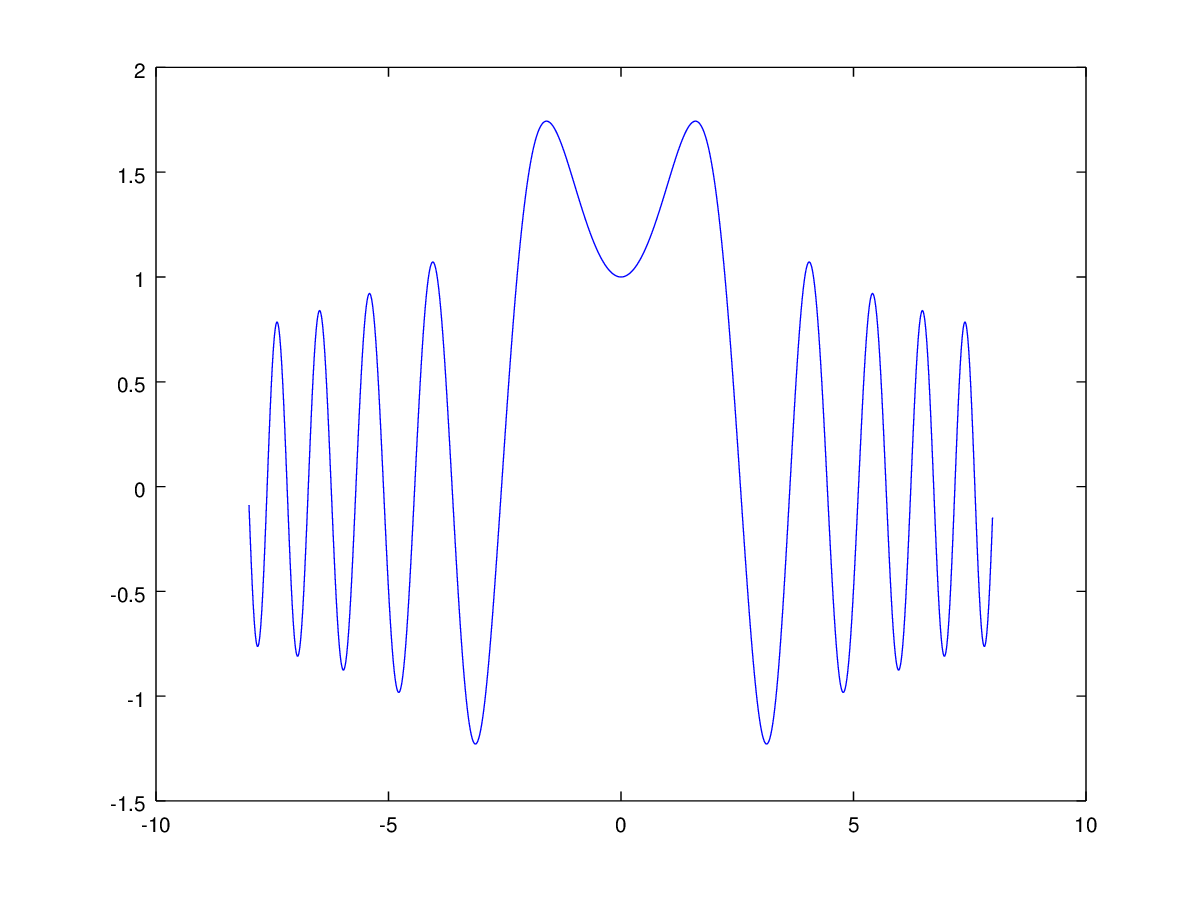
\includegraphics[scale=0.7]{./wellen/octave/images/welle.jpg}
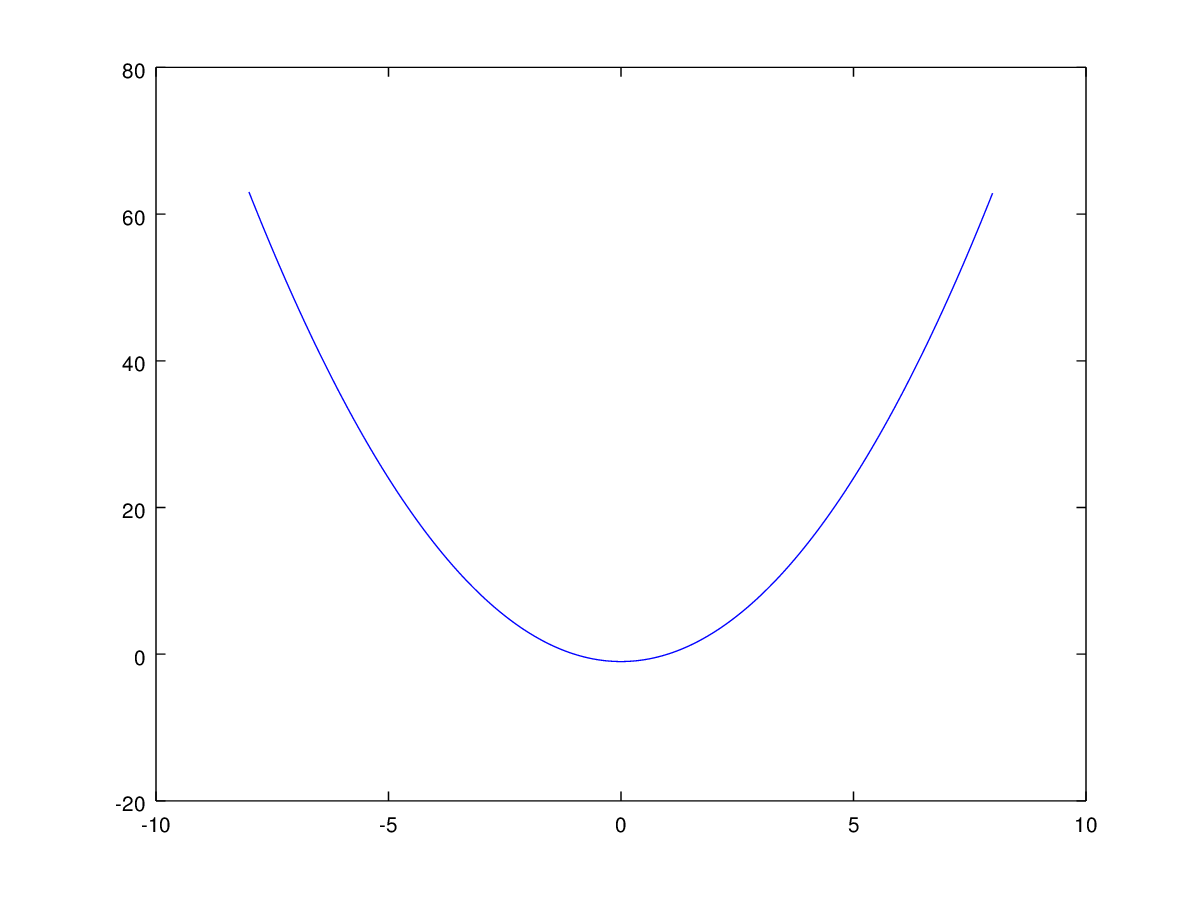
\includegraphics[scale=0.7]{./wellen/octave/images/parabel.jpg}

\clearpage
\section{Octave Code}
\lstinputlisting[style=Matlab]{./wellen/octave/ak.m}
\printbibliography[heading=subbibliography]
\end{refsection}